\chapter{基于混合对数正太模型SAR图像目标检测}
\label{cha:LMM}

\section{引言}
\label{sec:chap2:sec1}
在使用恒虚警率的SAR图像目标检测方法中,对海杂波的精准建模是其中至关重要的问题。目前可以有效
对海杂波建模的分布模型有锐利分布,K分布,威布尔分布,对数高斯分布等。在本章中我采用混合对数正太
模型对强度SAR图像中的海杂波进行建模,实质上对数混合正太模型(lognormal mixture model)等价于强度SAR图像在对数域上的混合
高斯模型,因此可以采用EM方法估计分布参数,得到海杂波概率密度分布后应用牛顿迭代法计算分割阈值输出
检测的结果图像


\section{混合对数正太模型}
\label{sec:chap2:sec2}
  定义强度SAR图像中的像素值$\bf{x}$为一随机变量,当其满足式\ref{equ:chap2:LMM}中的分布时,我们称随机变量$\bf{x}$
  服从包含K个成分的混合对数正太分布。

    \begin{equation}
      \label{equ:chap2:LMM}
      {f_x}(x) = \mathop \Sigma \limits_{i = 1}^K {\alpha _i} \cdot \frac{1}{{\sqrt {2\pi } {\sigma _i}x}}\exp ( - \frac{{{{(\ln x - {\mu _i})}^2}}}{{2{\sigma ^2}}}),x > 0
    \end{equation}
  在式\ref{equ:chap2:LMM}中,$\alpha_i$, $\mu_i$, $\sigma_i(i=1,2,...,K)$为混合对数正太分布参数
  其中$\alpha_i$权重系数满足式\ref{equ:chap2:weigth}所示关系。混合对数正太分布为K个对数正太分布
  加权求和。$\mu_i$,$\sigma_i$为各独立的对数正太分布参数。

    \begin{equation}
      \label{equ:chap2:weigth}
      \sum\limits_{i = 1}^K {{\alpha _i} = 1,{\alpha _i} \ge 0} 
    \end{equation}

  对随机变量$\bf{x}$做形式变换,另$Y=\bf{x}$,我们可以推导出对于随机变量$Y$,其满足的概率密度函数如式\ref{equ:chap2:GMM}所示,显然
  随机变量$Y$满足含有K个分量的混合高斯分布,等价来讲对于强度SAR图像采用混合对数正太模型对海杂波进行建模
  等价于在SAR图像对数强度域上应用混合高斯模型,因此在该建模方法中,首先对强度SAR图像取对数变换到对数域,然后应用混合高斯
  模型描述海杂波的分布。

    \begin{equation}
      \label{equ:chap2:GMM}
        {f_Y}(y) = \mathop \Sigma \limits_{i = 1}^K {\alpha _i} \cdot \frac{1}{{\sqrt {2\pi } {\sigma _i}}}\exp ( - \frac{{{{(y - {\mu _i})}^2}}}{{2{\sigma ^2}}})
    \end{equation}


  \section{海杂波分布参数估计}

      在\ref{sec:chap2:sec2}节表明,混合对数正太分布在强度域与混合高斯分布在对数域上等价,因此混合正太
      分布中的参数计算可以采用目前现有的混合高斯模型参数计算方法。在文献[4]中表明了对于混合高斯模型,最大期望算法
      是一种高效的估计混合高斯分布参数的方法。因此在参数估计中,应用EM算法计算海杂波分布参数。参数迭代更新如式\ref{equ:chap2:paramupdate}
      所示。在该式中$\phi (y|{\mu _k},{\sigma _k})$为均值为$\mu_k$,标准差为$\sigma_k$的高斯分布,$n$为参与估计的杂波像素数量,
      $y$为取对数后的图像强度值。      

    \begin{equation}
      \label{equ:chap2:paramupdate}
      \begin{array}{*{20}{c}}
        {{\mu _k}^{i + 1} = \frac{{\sum\limits_{j = 1}^n {{\gamma _{jk}}{y_j}} }}{{\sum\limits_j^n {{\gamma _{jk}}} }}}\\
        {{\sigma _k}^{{\rm{i}} + 1} = \sqrt {\frac{{\sum\limits_{j = 1}^n {{\gamma _{jk}}({y_j} - {\mu _k}^{i + 1})} }}{{\sum\limits_j^n {{\gamma _{jk}}} }}} }\\
        {{\alpha _k}^{i + 1} = \frac{{\sum\limits_j^n {{\gamma _{jk}}} }}{n}}\\
        {{\gamma _{jk}} = \frac{{{\alpha _k}^i\phi ({y_j}|u_k^i,\sigma _k^i)}}{{\sum\limits_{k = 1}^K {{\alpha _k}^i\phi ({y_j}|u_k^i,\sigma _k^i)} }}}
      \end{array}
    \end{equation}

    受自然条件风速、风向的影响,同一SAR图像不同区域的杂波分布不尽相同,因此采用图\ref{fig:chap2:slide}所示的
    滑动窗进行局部杂波像素的选取,该滑动窗分为三个区域分别为检测像素区域,保护区域,杂波区域。合适大小的保护区域可以减少
    舰船目标像素对杂波统计分布参数估计的干扰。选定杂波像素值后,将其代入到式\ref{equ:chap2:paramupdate}中进行
    海杂波分布参数的迭代估计。

    \begin{figure}[H] % use float package if you want it here
      \centering
      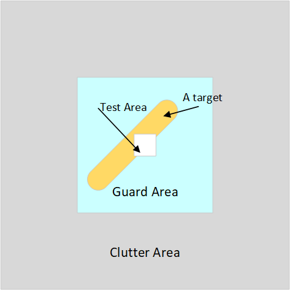
\includegraphics[width=0.5\textwidth]{slide.png}
      \caption{采用滑动窗进行自适应杂波参数估计,阴影所示像素用于杂波估计}
      \label{fig:chap2:slide}
    \end{figure}   
\section{应用LMM模型进行CFAR舰船检测}
    当采用混合对数正太模型对海杂波分布进行建模后,根据给定的恒虚警率来实现CFAR方法检测。检测阈值通过
    式\ref{equ:chap2:detecthres}来得到,该式中T为恒虚警率所对应的检测阈值,$f(x)$为采用局部海杂波像素估计
    得到的混合对数正太分布,$F(x)$为$f(x)$对应的累积密度分布函数。我们采用牛顿迭代法来解决这个非线性的
    等式方程,迭代更新公式如式\ref{equ:chap2:newtonupdate}所示,迭代停止的条件为$\left| {{T_{i + 1}} - {T_i}} \right| < \delta$
    当满足迭代精度要求后,最终的检测阈值为${T^*} = {T_{i + 1}}$。

    \begin{equation}
      \label{equ:chap2:detecthres}
      {{\rm{P}}_{FA}} = \int_T^{ + \infty } {f(x)dx = 1 - F(x)}
    \end{equation}

    \begin{equation}
      \label{equ:chap2:newtonupdate}
      {{\rm{T}}_{i + 1}} = {T_i} - \frac{{F({T_i}) + {P_{FA}} - 1}}{{f({T_i})}}
    \end{equation}

    在\ref{sec:chap2:sec2}节,我们证明LMM模型等价于对数域的混合高斯模型,$f(x)$的概率密度函数在对数变换后可表示为式\ref{equ:chap2:GMM}
    的形式。混合高斯分布的累积概率密度函数可以表示为式\ref{equ:chap2:erf}。其中$erf(x)$为误差函数,可以通过查表的方法
    来得到误差函数的值从而减少计算量。

    \begin{equation}
      \label{equ:chap2:erf}
      F(x) = \frac{1}{2}\sum\limits_{i = 1}^K {{\lambda _k}[1 + erf(\frac{{x - {u_i}}}{{\sqrt 2 {\sigma _i}}})]}
    \end{equation}

    综合前几节所述,使用混合对数正太模型的CFAR舰船目标检测流程如算法\ref{alg:chap2:LMM}所示

    \begin{algorithm}[t]
      \caption{基于LMM分布的CFAR舰船检测算法}
      \label{alg:chap2:LMM}
      \KwIn{HH通道强度SAR图像}
      \BlankLine
      初始化,将强度图像做对数变换得到对数域强度图像,设置滑动窗的参数。

      \ForEach{图像中的像素}{
          从对数强度图像中根据滑动窗选择海杂波像素值$\bf{y}$

          采用EM迭代算法计算LMM分布参数$\mu_i$,$\alpha_i$与$\sigma_i$

          根据式\ref{equ:chap2:newtonupdate}计算检测阈值$T$

          如果$y(i,j)>T$则该像素点为舰船目标像素点,否则为背景杂波像素点。
      }
      \KwOut{二值舰船检测结果图像$result$}  
    \end{algorithm}

\section{GPU算法优化}
    通常应用滑动窗的SAR图像目标检测方法都面临着计算复杂度高,时间效率低等问题。而滑动窗参数估计是一类典型的
    可以采用并行方式去计算的问题,不同滑动窗之间所用数据和输出结果是相互独立的,没有依赖与调用关系,因此可以
    将滑动穿参数估计部分在GPU多线程上去执行。

    在估计LMM分布参数的过程中,要进行多次迭代并访问杂波像素值来更新分布参数,因此减少此部分数据访存时间可以
    大幅提升算法的运行效率,对于GPU而言总主要有以下几种存储类型,一、二级缓存,寄存器,全局内存,共享内存,纹理内存,
    常量内存。其中一二级缓存为不可编程的存储介质,系统运行时环境会自动分配数据在其上的位置以获得更加优良的性能。对于可编程
    存储介质,通常每个线程的寄存器数量非常有限,因此不适合存储海杂波像素值。而全局内存、常量内存与纹理内存是板上内存,访问延
    迟相较于片上的共享内存要高20~30倍。因此我们选择片上的共享内存作为海杂波像素的高速暂存存储器,通过访问共享内存上的杂波像素,
    可以优化全局内存访问的模式,从而提升核函数的执行速度。

     \begin{figure}[H] % use float package if you want it here
      \centering
      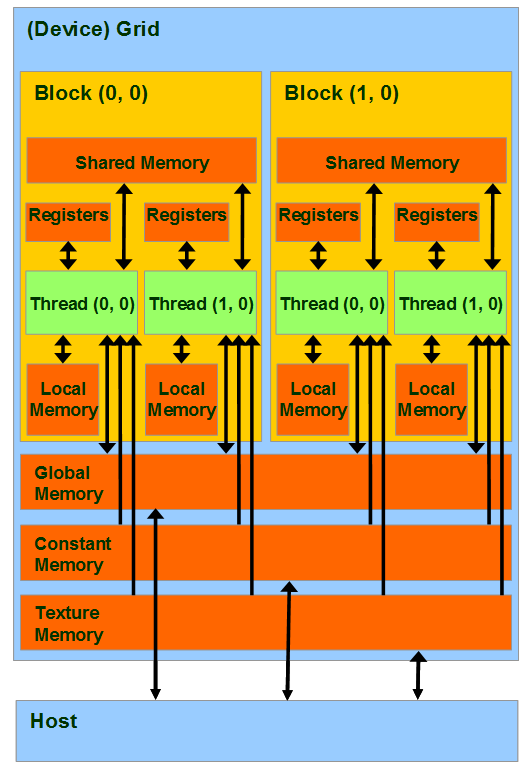
\includegraphics[width=0.5\textwidth]{memory.png}
      \caption{CUDA内存模型}
      \label{fig:chap2:slide}
    \end{figure}   

    共享内存得容量有限,通常为64KB。该存储空间位于流多处理器上类似于CPU的一级缓存,此内存空间被一个线程块中的
    所有线程共享。要合理的设置线程块的大小,避免因共享内存空间过度使用导致活跃线程束减少从而影响程序的执行效率。
    结合滑动窗的大小,我们最终将线程块的大小设置为8x8,将线程网格的大小设置为$(\left\lfloor {\frac{{w + 1}}{8}} \right\rfloor ,\left\lfloor {\frac{{h + 1}}{8}} \right\rfloor )$
    。其中$\left\lfloor {} \right\rfloor $代表向下取整,$w$代表SAR图像的宽度,$h$代表SAR图像的高度。
    
    在分配好线程块与线程网格大小后,每个线程与SAR图像像素索引对应关系为:row = threadIdx.x + blockDim.x * blockIdx.x; column = threadIdx.y + blockDim.y * blockIdx.y;
    之后根据滑动窗,将检测像素所对应的海杂波像素复制到该线程所对应的共享内存内存空间,在EM算法过程中在共享内存中读取杂波像素值进行分布
    的参数更新,当满足参数迭代停止条件后得到LMM分布参数,然后应用牛顿迭代法计算检测阈值$T$,当检测像素值大于阈值$T$时,
    该像素被标记为舰船目标像素。当所有线程执行完毕后,将检测结果从设备内存拷贝至主机内存,进行进一步的分析与处理。

    \begin{figure}[H] % use float package if you want it here
      \centering
      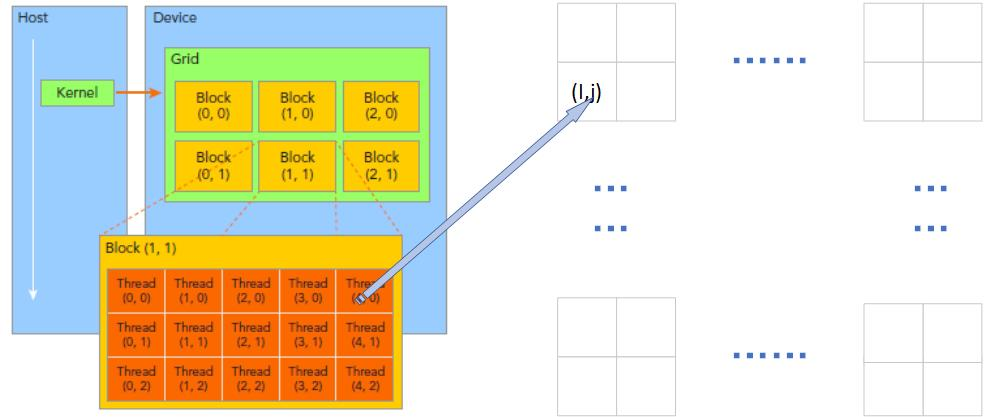
\includegraphics[width=0.9\textwidth]{map.jpg}
      \caption{CUDA线程与检测像素映射关系}
      \label{fig:chap2:slide}
    \end{figure} 

\section{LMM实验结果}
    本次实验中我们使用的是由星载成像雷达系统(SIR-C/X)拍摄的香港维多利亚港的SAR图像数据。SAR图像部分HH通道
    强度图像如图\ref{fig:chap2:source}所示


  \begin{figure}[h]
    \centering%
    \begin{subfigure}{0.4\textwidth}\
      \includegraphics[width=5cm]{HongKong1.png}
    \end{subfigure}%
    \begin{subfigure}{0.4\textwidth}
      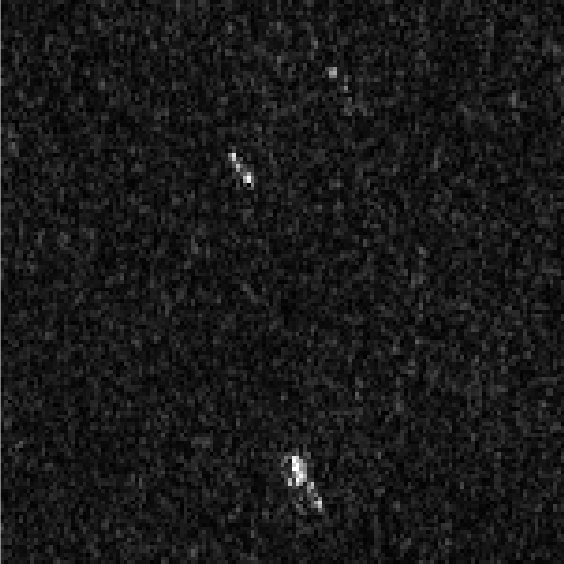
\includegraphics[width=5cm]{HongKong2.png}
    \end{subfigure}

    \begin{subfigure}{0.4\textwidth}
      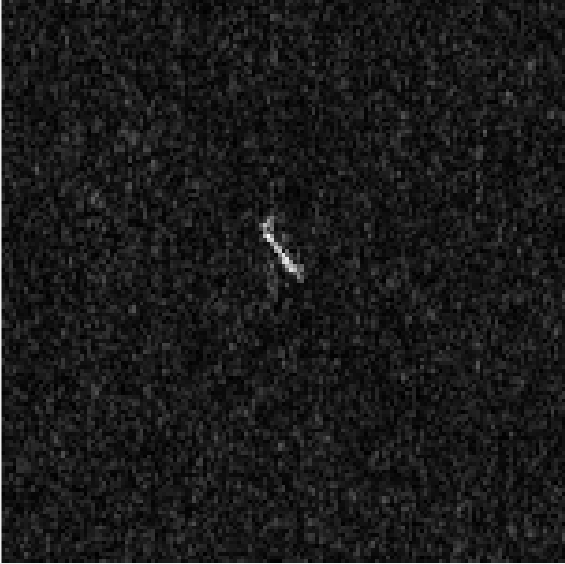
\includegraphics[height=5cm]{HongKong3.png}
    \end{subfigure}%
    \begin{subfigure}{0.4\textwidth}
      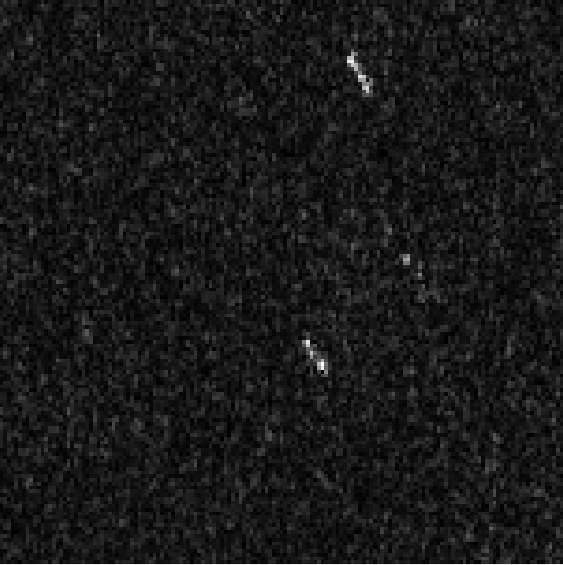
\includegraphics[height=5cm]{HongKong4.png}
    \end{subfigure}   

    \caption{四张SIR-C/XSAR强度图像}
    \label{fig:chap2:source}
  \end{figure}

  在检测中我们设置恒虚警为$1x10^{-5}$,检测结果如图\ref{fig:chap2:detectresult}所示,其中白色区域代表舰船目标像素区域,
  黑色区域代表背景杂波区域,从结果可以看出在给定的虚警率下LMM算法对目标像素与舰船像素作做出了正确的
  分割。本次实验使用的GPU为NVIDIA TITAN V,经过多次实验验证,相较于使用单线程CPU的检测方法,程序运行的时间效率提升了近21倍,
  不同平台运行时间如表所示,原始SAR图像中的舰船数量较少,检测结果中虚警漏报的数量均为0,准确率达到了$100\%$。

  \begin{figure}[h]
    \centering%
    \begin{subfigure}{0.4\textwidth}\
      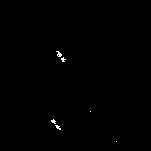
\includegraphics[width=5cm]{HongKong1r.jpg}
    \end{subfigure}%
    \begin{subfigure}{0.4\textwidth}
      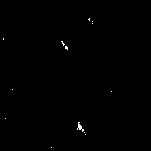
\includegraphics[width=5cm]{HongKong2r.jpg}
    \end{subfigure}

    \begin{subfigure}{0.4\textwidth}
      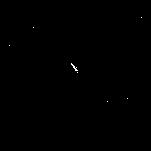
\includegraphics[height=5cm]{HongKong3r.jpg}
    \end{subfigure}%
    \begin{subfigure}{0.4\textwidth}
      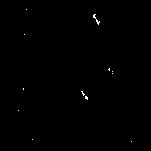
\includegraphics[height=5cm]{HongKong4r.jpg}
    \end{subfigure}   

    \caption{LMM检测结果}
    \label{fig:chap2:detectresult}
  \end{figure}

  \begin{table}[htb]
  \centering
    \begin{minipage}[t]{1\linewidth} % 如果想在表格中使用脚注,minipage是个不错的办法
    \caption[LMM算法时间]{串行与并行LMM算法运行时间对比}
    \label{tab:chap3:timeresult}
      \begin{tabularx}{\linewidth}{lXX}
        \toprule[1.5pt]
        {\heiti 检测算法} & {\heiti 运行平台} & {\heiti 运行时间/s} \\ \midrule[1pt]
        LMM-CFAR(Matlab单线程) & (Intel(R) i7-9750H CPU) & 15.1 \\
        LMM-CFAR(GPU多线程) &  GPU(Titan V) & 0.73 \\
        \bottomrule[1.5pt]
      \end{tabularx}
    \end{minipage}
  \end{table}

\section{小结}
    本章我们实现了基于混合对数正太分布的恒虚警率SAR图像舰船检测方法,在本质上混合对数分布等价于
    强度SAR图像在对数域上的混合高斯分布,因此采用了EM算法与牛顿迭代法得到分布参数与检测阈值。对于滑动窗
    参数估计的部分,我们将其放置在GPU上进行并行计算,并使用延迟更低的共享内存来加快访存速度。相较于传统的
    串行解决方案,本章基于GPU的LMM方法不仅在时间性能获得了显著的提升同时还保证了检测效果的有效性。


